\def\QRCODE{TB_image_TUT.IMG.introduction_matlabqrcode.png}
\def\QRPAGE{http://www.iptutorials.science/tree/master/TB_image/TUT.IMG.introduction/matlab}
\mcorrectionsection{Matlab correction}


\subsection{First manipulations}

The following function is usefull to display 4 images:
\begin{matlab}
function affichePar4(A, B, C, D)
% Display 4 images in the same window
figure();
subplot(2,2,1);
imshow(A);

subplot(2,2,2);
imshow(B);

subplot(2,2,3);
imshow(C);

subplot(2,2,4);
imshow(D);
\end{matlab}

\subsubsection{Load and save image}
\begin{matlab}
I=imread('retine.png');
imagesc(I);
figure(2);
imshow(I);

% data inside image
imfinfo('retine.png');
size(I)
\end{matlab}

\begin{mwindow}
>> imfinfo('retine.png')
ans = 
                  Filename: '/home/yann/Documents/Cou...'
               FileModDate: '05-Nov-2013 12:04:24'
                  FileSize: 741963
                    Format: 'png'
             FormatVersion: []
                     Width: 922
                    Height: 911
                  BitDepth: 24
                 ColorType: 'truecolor'
           FormatSignature: [137 80 78 71 13 10 26 10]
                  Colormap: []
                 Histogram: []
             InterlaceType: 'none'
              Transparency: 'none'
    SimpleTransparencyData: []
           BackgroundColor: []
           RenderingIntent: []
            Chromaticities: []
                     Gamma: []
               XResolution: 2835
               YResolution: 2835
            ResolutionUnit: 'meter'
                   XOffset: []
                   YOffset: []
                OffsetUnit: []
           SignificantBits: []
              ImageModTime: []
                     Title: []
                    Author: []
               Description: []
                 Copyright: []
              CreationTime: []
                  Software: []
                Disclaimer: []
                   Warning: []
                    Source: []
                   Comment: []
                 OtherText: []
>> 
\end{mwindow}

\subsubsection{JPEG file format}
\index{File formats}

JPEG is a compressed file format that accept loss in quality. The following code illustrates the different quality parameters, shown in Fig.\ref{fig:introduction:matlab:lossy}.

\begin{matlab}
% test read/write with loss in quality
imwrite(I, 'retine_lossy_25.jpg', 'jpg', 'Mode', 'lossy', 'Quality', 25);
a1=imread('retine_lossy_25.jpg');

imwrite(I, 'retine_lossy_50.jpg', 'jpg', 'Mode', 'lossy', 'Quality', 50);
a2=imread('retine_lossy_50.jpg');

imwrite(I, 'retine_lossy_75.jpg', 'jpg', 'Mode', 'lossy', 'Quality', 75);
a3=imread('retine_lossy_75.jpg');

imwrite(I, 'retine_lossy_100.jpg', 'jpg', 'Mode', 'lossy', 'Quality', 100);
a4=imread('retine_lossy_100.jpg');

% zoom in particular area
d1=imcrop(a1, [75 68 130 112]);
d2=imcrop(a2, [75 68 130 112]);
d3=imcrop(a3, [75 68 130 112]);
d4=imcrop(a4, [75 68 130 112]);

affichePar4(d1, d1, d3, d4);
\end{matlab}

\begin{figure}[htbp]
 \centering
 \subfloat[Quality: 100.]{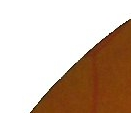
\includegraphics[width=5cm]{retine_crop_100.png}}\hfill
 \subfloat[Quality: 75.]{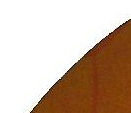
\includegraphics[width=5cm]{retine_crop_75.png}}
 
 \subfloat[Quality: 50.]{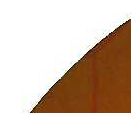
\includegraphics[width=5cm]{retine_crop_50}}\hfill
 \subfloat[Quality: 25.]{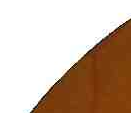
\includegraphics[width=5cm]{retine_crop_25}}
 
 \caption{Illustration of different quality parameters used in JPEG compression. The original image is zoomed in order to emphasize the quality loss.}
 \label{fig:introduction:matlab:lossy}
\end{figure}


\subsection{Image histogram}
\index{Histogram}

Notice that \matlabregistered{} indices begin at 1!

\begin{matlab}
function h=myHist(image)
% histogram function of grayscale image coded in 8 bits
h=zeros(256, 1);

for i=1:size(image, 1)
	for j=1:size(image, 2)
		h(image(i,j)+1) = h(image(i,j)+1) + 1;
	end
end
\end{matlab}

This is the \matlabregistered{} version.
\begin{matlab}
muscle=imread('muscle.jpg');
h = imhist(muscle);
figure();plot(h);
\end{matlab}

\subsection{Linear mapping of the image intensities}
The application of a linear stretching is quite simple. The histograms are illustrated in Fig.\ref{fig:introduction:matlab:histo_stretched}.

\begin{matlab}
cornea=imread('cellules_cornee.jpg');
minimum = min(cornee(:));
maximum = max(cornee(:));

a=255/(maximum-minimum);
b=-255*minimum/(maximum-minimum);

cornee2 = a*cornee + b;
figure();
subplot(2,2,1);imshow(cornee); title('cornea');
subplot(2,2,2);imshow(cornee2);title('stretched cornea');

% histograms
subplot(2,2,3);plot(imhist(cornee)); title('histogram of cornea');
subplot(2,2,4);plot(imhist(cornee2));title('stretched histogram');
\end{matlab}

\begin{figure}[htbp]
 \centering
 \subfloat[Original image.]{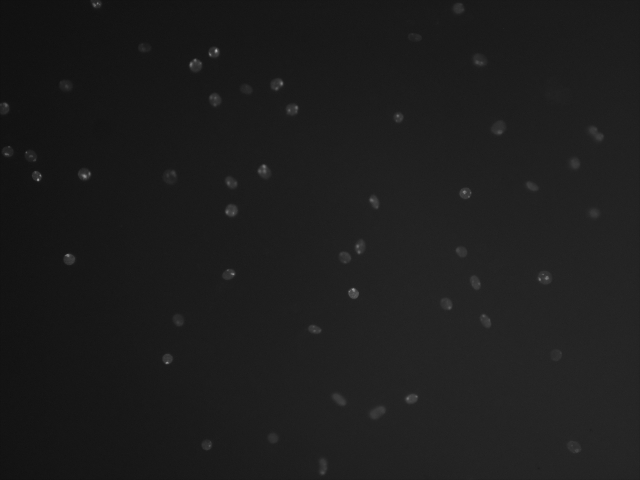
\includegraphics[width=5cm]{cellules_cornee.jpg}}\vspace{.5cm}
 \subfloat[Histogram of the image cellules\_cornee.]{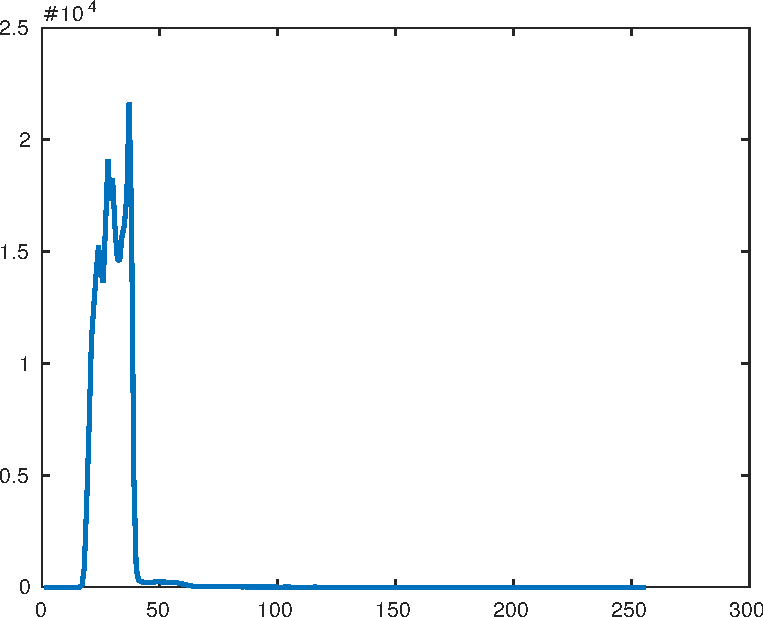
\includegraphics[width=5cm]{hist_cornee.pdf}}\vspace{.5cm}
 \subfloat[Stretched histogram.]{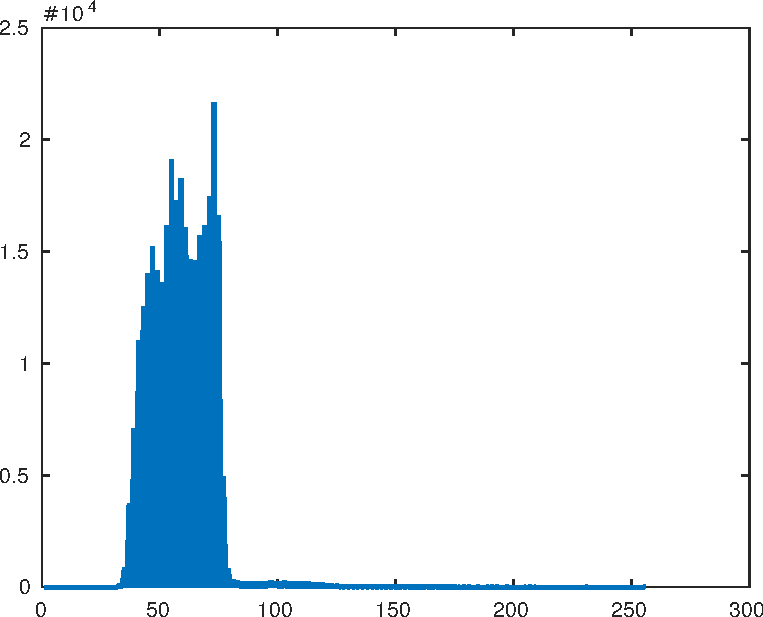
\includegraphics[width=5cm]{hist_cornee_stretched.pdf}}
 \caption{Result of histogram stretching.}
 \label{fig:introduction:matlab:histo_stretched}
\end{figure}


\subsection{Color quantization}

\index{Quantization}

The objective is to reduce the number of colors by 2 (for example). We use the 
properties of the data types: integer type rounds automatically while dividing.
In the proposed example, the gray value is taken as the green channel of a color retina image (Fig.\ref{fig:introduction:matlab:quantification}).

\begin{matlab}
image_gris = I(:,:,2); % green channel
q4=image_gris/4*4;
q16=image_gris/16*16;
q32=image_gris/32*32;
affichePar4(image_gris, q4, q16, q32);
\end{matlab}

\begin{figure}[htbp]
 \centering
 \subfloat[Original retina image, green channel.]{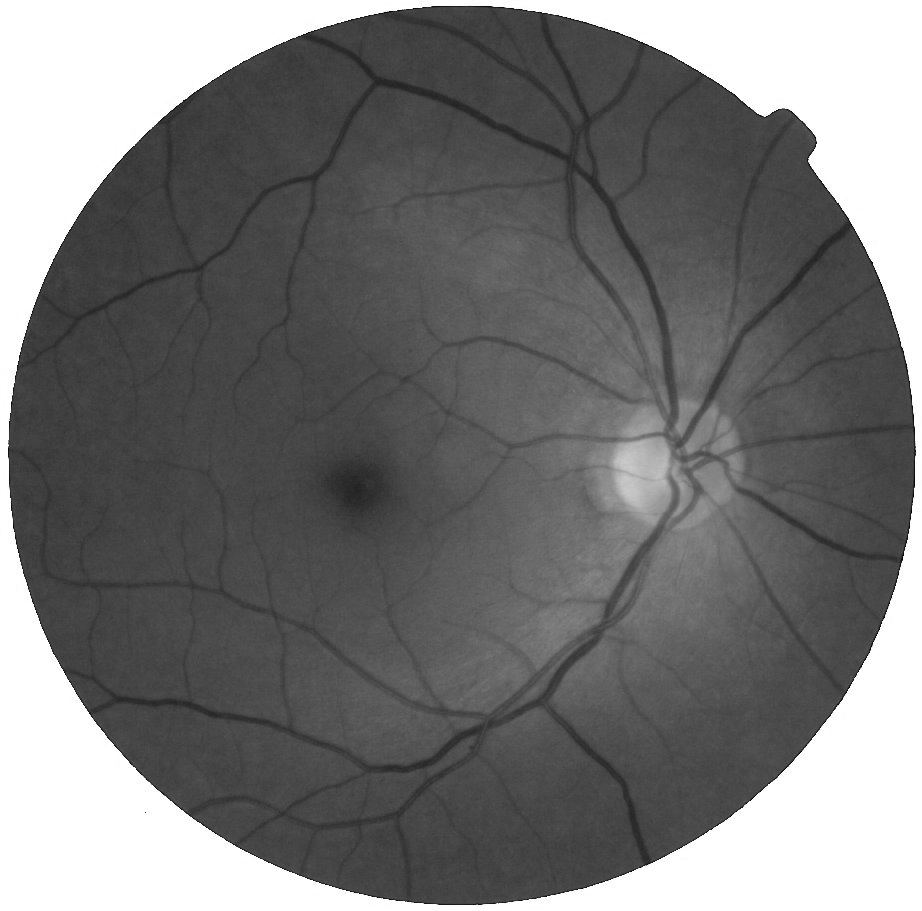
\includegraphics[width=5cm]{origine_green.png}}
 \subfloat[64 grey levels.]{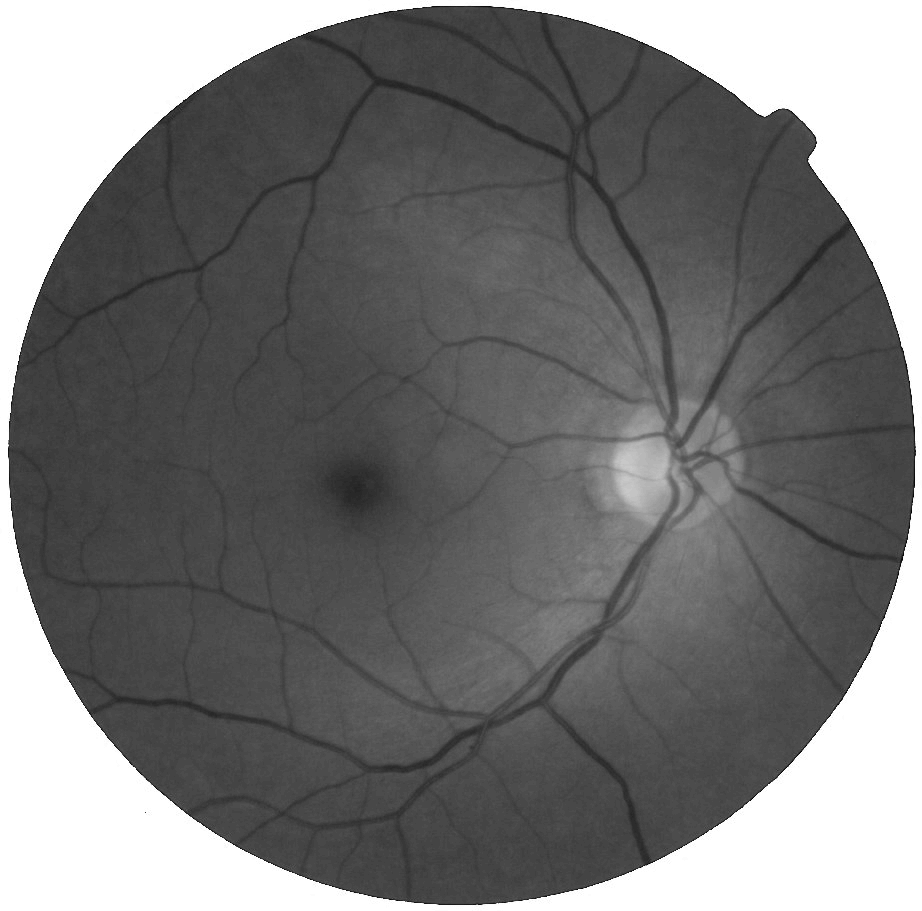
\includegraphics[width=5cm]{quantification_q4.png}}
 
 \subfloat[16 grey levels.]{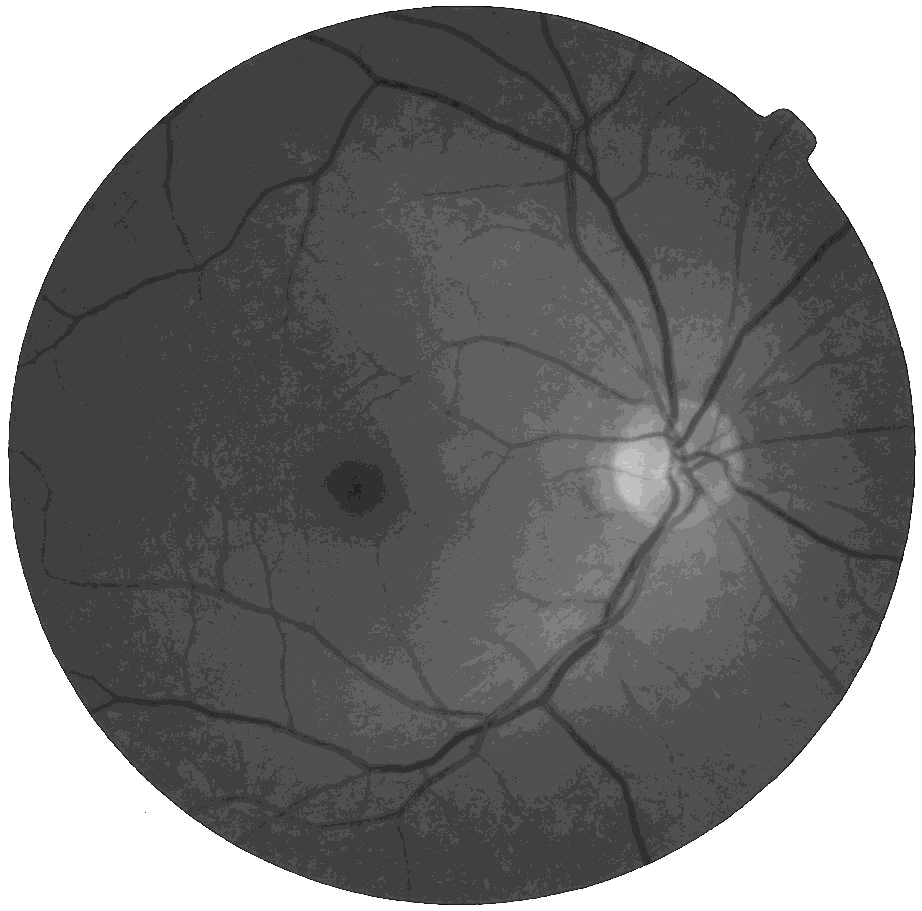
\includegraphics[width=5cm]{quantification_q16}}
 \subfloat[8 grey levels.]{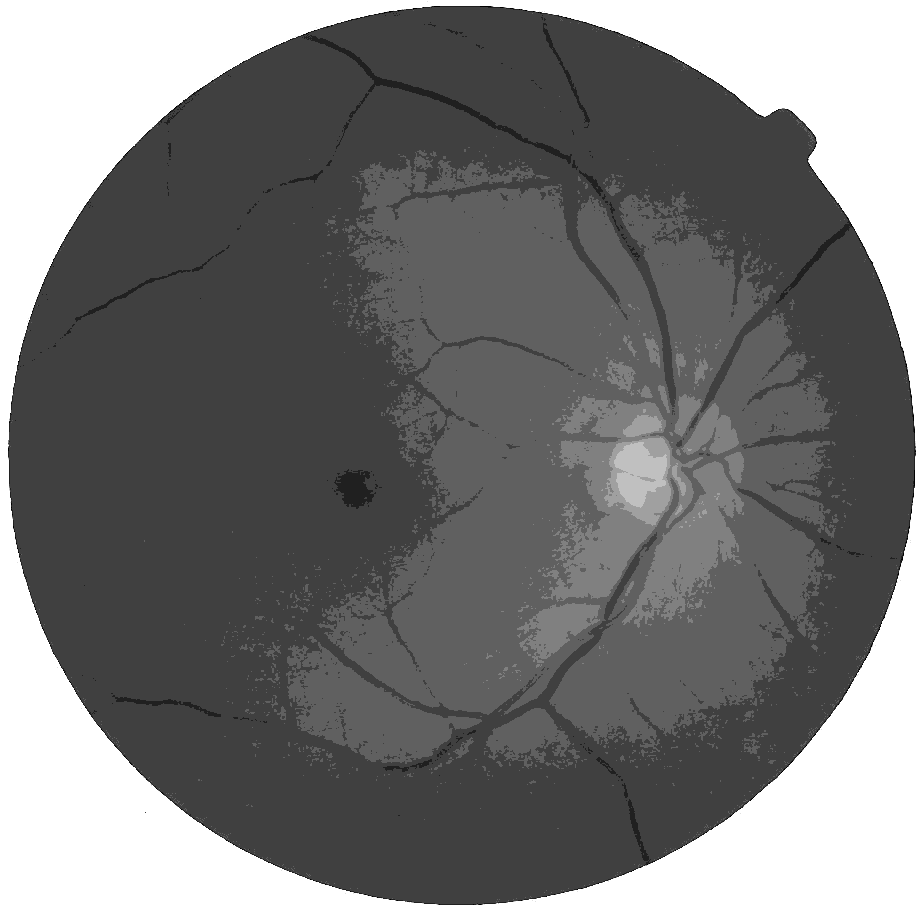
\includegraphics[width=5cm]{quantification_q32}}
 
 \caption{Illustration of different quality parameters used in JPEG compression.}
 \label{fig:introduction:matlab:quantification}
\end{figure}


\subsection{Aliasing (Moir\'e) effect}\index{Aliasing}
The aliasing effect occurs when two sampling are performed. This is illustrated in Fig.\ref{fig:introduction:matlab:moire} with the following code.

\begin{matlab}
function C=cercle(fs,f)
% Generates an image with aliasing effect
% fs: sample frequency
% f : signal frequency

% time sampling
t=0:1/fs:1;

C=zeros(size(t,2));
for i=1:size(t,2);
    for j=1:size(t,2);
        C(i,j)=sin(2*pi*f*sqrt(t(i)^2+t(j)^2));
    end
end
\end{matlab}

\begin{figure}[htbp]
 \centering
 
 \subfloat[$f_s=300, f=50$.]{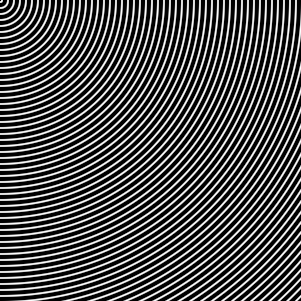
\includegraphics[width=5cm]{moire_1.png}}
 \hspace{1cm}
 \subfloat[$f_s=80, f=50$.]{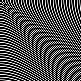
\includegraphics[width=5cm]{moire_2.png}}
 
 \caption{Illustration of the aliasing effect.}
 \label{fig:introduction:matlab:moire}
\end{figure}



\subsection{Low-pass filtering}\index{Filtering!Low-pass}

The mean and Gaussian filters are linear filters. Other filters are called rank filters. See Fig.\ref{fig:introduction:matlab:lpfilters} for an illustration.
\begin{matlab}
% read image and convert to double for convolution computation
A=imread('bloodCells.bmp');
A=double(A)/255;

% display images
figure;
subplot(231);imshow(A);title('Original');

Amin=ordfilt2(A,1,ones(5,5),'symmetric');
subplot(232);imshow(Amin);title('Low-pass filter : min');

Amax=ordfilt2(A,25,ones(5,5),'symmetric');
subplot(233);imshow(Amax);title('Low-pass filter : max');

Amoyen=imfilter(A,1/25*ones(5,5),'symmetric');
subplot(234);imshow(Amoyen);title('Low-pass filter : moyen');

Amedian=ordfilt2(A,13,ones(5,5),'symmetric');
subplot(235);imshow(Amedian);title('Low-pass filter : median');

hgauss=fspecial('gaussian',[5 5],1);
Agauss=imfilter(A,hgauss);
subplot(236);imshow(Agauss);title('Low-pass filter : gaussien');
\end{matlab}

\begin{figure}[htbp]
 \centering
 
 \subfloat[Minimum filter.]{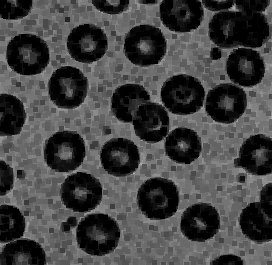
\includegraphics[width=5cm]{bloodcells_min.png}}
 \hspace{1cm}
 \subfloat[Maximum filter.]{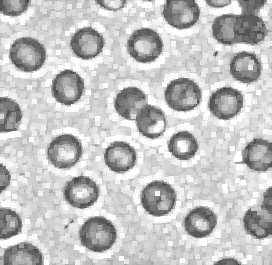
\includegraphics[width=5cm]{bloodcells_max.png}}
 
 \subfloat[Mean filter.]{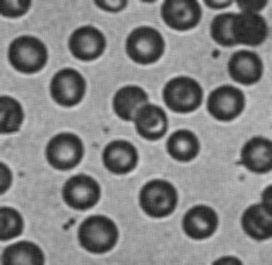
\includegraphics[width=5cm]{bloodcells_moyen.png}}
 \hspace{1cm}
 \subfloat[Median filter.]{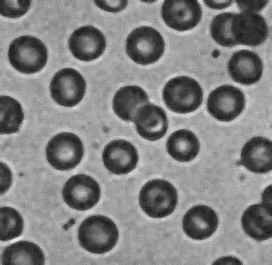
\includegraphics[width=5cm]{bloodcells_median.png}}
 
 \subfloat[Gaussian filter, $\sigma=1$.]{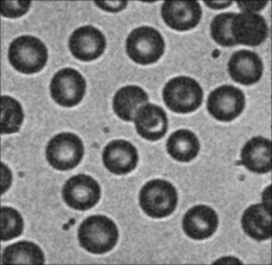
\includegraphics[width=5cm]{bloodcells_gauss.png}}
 \hspace{1cm}
 \subfloat[Original image.]{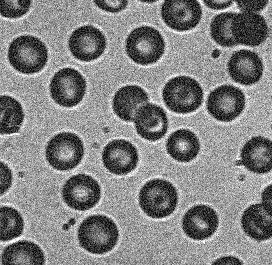
\includegraphics[width=5cm]{bloodCells.png}}

 \caption{Low-pass filters computed in a $5\times 5$ neighborhood.}
 \label{fig:introduction:matlab:lpfilters}
\end{figure}

\newpage
\subsection{High pass filters}
\index{Filtering!High-pass}
These high-pass filters are simple the difference (residu) between the original image and a low-pass filter (Fig.\ref{fig:introduction:matlab:hpfilters}).

\begin{matlab}
figure;
subplot(231);imshow(A);title('Original');

AminPH=A-Amin;
subplot(232);imshow(AminPH);title('High-pass : min');

AmaxPH=Amax-A;
subplot(233);imshow(AmaxPH);title('High-pass : max');

AmoyenPH=A-Amoyen;
subplot(234);imshow(AmoyenPH);title('High-pass : moyen');

AmedianPH=A-Amedian;
subplot(235);imshow(AmedianPH);title('High-pass : median');

AgaussPH=A-Agauss;
subplot(236);imshow(AgaussPH);title('High-pass : gaussien');
\end{matlab}

\begin{figure}[htbp]
 \centering
 
 \subfloat[Residu from minimum filter.]{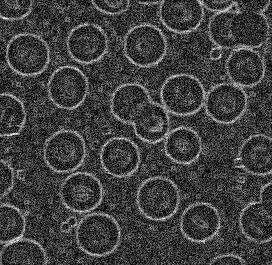
\includegraphics[width=5cm]{bloodcells_hpmin.png}}
 \hspace{1cm}
 \subfloat[Residu from maximum filter.]{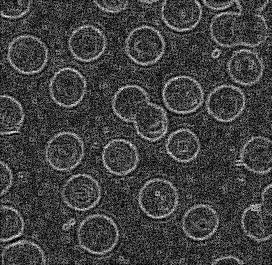
\includegraphics[width=5cm]{bloodcells_hpmax.png}}
 
 \subfloat[Residu from mean filter.]{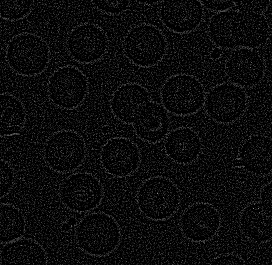
\includegraphics[width=5cm]{bloodcells_hpmoyen.png}}
 \hspace{1cm}
 \subfloat[Residu from median filter.]{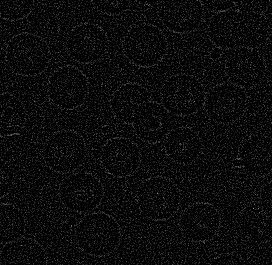
\includegraphics[width=5cm]{bloodcells_hpmedian.png}}
 
 \subfloat[Residu from Gaussian filter, $\sigma=1$.]{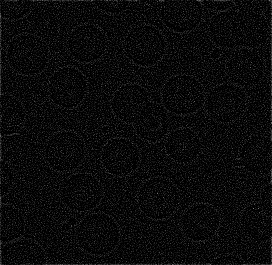
\includegraphics[width=5cm]{bloodcells_hpgauss.png}}
 \hspace{1cm}
 \subfloat[Original image.]{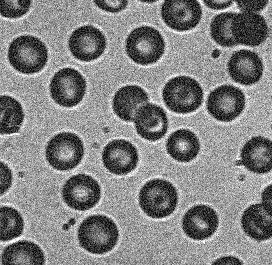
\includegraphics[width=5cm]{bloodCells.png}}

 \caption{High-pass filters computed in a $5\times 5$ neighborhood.}
 \label{fig:introduction:matlab:hpfilters}
\end{figure}

\subsubsection{Laplacian filter}\index{Laplacian}
The Laplacian filter is based on the second derivative (Fig.\ref{fig:introduction:matlab:laplacian}).
\begin{matlab}
B=imread('osteoblaste.bmp');
B=double(B);
B=B/255;
hlaplacien=[-1 -1 -1; -1 8 -1;-1 -1 -1];
Blaplacien=imfilter(B,hlaplacien);
Alaplacien=imfilter(A,hlaplacien);
figure;
subplot(221);imshow(A);title('original image');
subplot(222);imshow(Alaplacien);title('Laplacian filter');
subplot(223);imshow(B);title('originale image');
subplot(224);imshow(Blaplacien);title('Laplacian filter');
\end{matlab}

\begin{figure}[htbp]
 \centering
 
 \subfloat[Laplacian filter.]{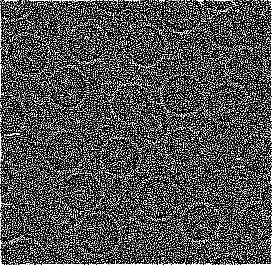
\includegraphics[width=5cm]{bloodcells_laplacian.png}}
 \hspace{1cm}
 \subfloat[Original image.]{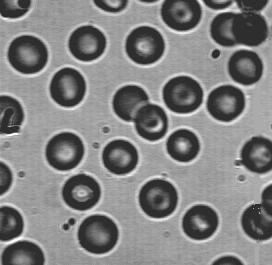
\includegraphics[width=5cm]{blood.jpg}}
 
 \subfloat[Laplacian filter.]{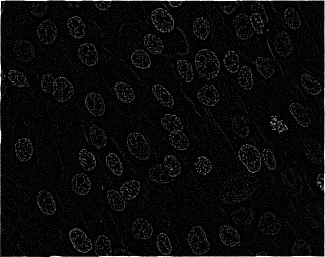
\includegraphics[width=5cm]{osteoblasts_laplacian.png}}
 \hspace{1cm}
 \subfloat[Original image.]{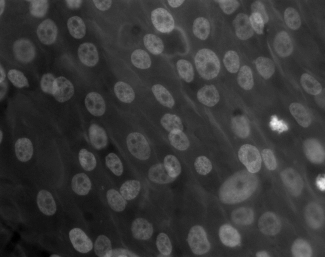
\includegraphics[width=5cm]{osteoblaste.png}}
 
 \caption{Laplacian filters.}
 \label{fig:introduction:matlab:laplacian}
\end{figure}

\newpage
\subsection{Derivative filters}
\subsubsection{Derivation: Prewitt gradient}
A gradient is a vector of the first derivatives. The norm of this vector represents the intensity of the contours (Fig.\ref{fig:introduction:matlab:prewitt} for the Prewitt gradient, and \ref{fig:introduction:matlab:sobel} for the Sobel gradient).
A derivative filter is very sensitive to noise.

\begin{matlab}
hprewittx=[-1 0 1;-1 0 1;-1 0 1];
hprewitty=hprewittx';
Aprewittx=imfilter(A,hprewittx);
Aprewitty=imfilter(A,hprewitty);
Aprewittxy=(Aprewittx.^2+Aprewitty.^2).^(0.5);
subplot(221);imshow(A);title('Original');
subplot(222);imshow(Aprewittxy);title('Prewitt : x and y');
subplot(223);imshow(Aprewittx);title('Prewitt : x');
subplot(224);imshow(Aprewitty);title('Prewitt : y');
\end{matlab}

\begin{figure}[htbp]
 \centering
 
 \subfloat[Horizontal direction.]{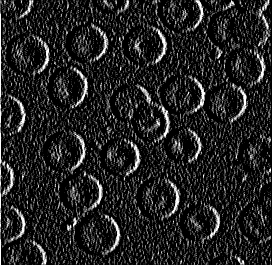
\includegraphics[width=5cm]{bloodcells_prewitt_x.png}}
 \hspace{1cm}
 \subfloat[Vertical direction.]{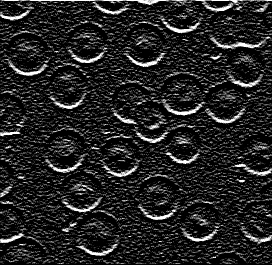
\includegraphics[width=5cm]{bloodcells_prewitt_y.png}}
 
 \subfloat[Norm of the gradient.]{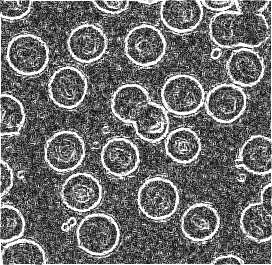
\includegraphics[width=5cm]{bloodcells_prewitt.png}}
 \hspace{1cm}
 \subfloat[Original image.]{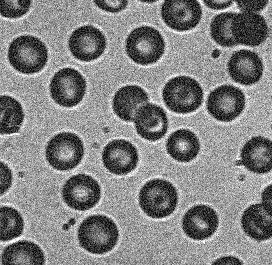
\includegraphics[width=5cm]{bloodCells.png}}

 \caption{Prewitt derivative filter.}
 \label{fig:introduction:matlab:prewitt}
\end{figure}

\subsubsection{Derivation: Sobel gradient}
\begin{matlab}
figure
hsobelx=[-1 0 1;-2 0 2;-1 0 1];
hsobely=hsobelx';
Asobelx=imfilter(A,hsobelx);
Asobely=imfilter(A,hsobely);
Asobelxy=(Asobelx.^2+Asobely.^2).^(0.5);
subplot(221);imshow(A);title('Original');
subplot(222);imshow(Asobelxy);title('Sobel : x and y');
subplot(223);imshow(Asobelx);title('Sobel : x');
subplot(224);imshow(Asobely);title('Sobel : y');
\end{matlab}

\begin{figure}[htbp]
 \centering
 
 \subfloat[Horizontal direction.]{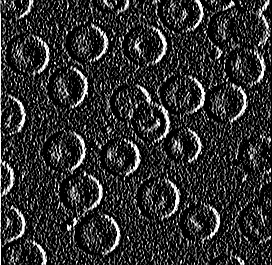
\includegraphics[width=5cm]{bloodcells_sobel_x.png}}
 \hspace{1cm}
 \subfloat[Vertical direction.]{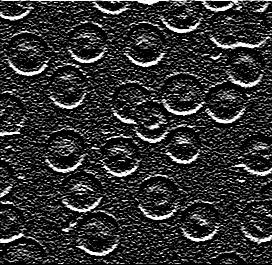
\includegraphics[width=5cm]{bloodcells_sobel_y.png}}
 
 \subfloat[Norm of the gradient.]{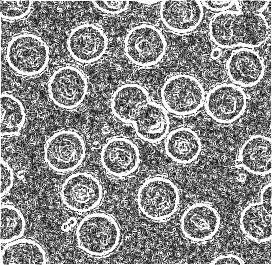
\includegraphics[width=5cm]{bloodcells_sobel.png}}
 \hspace{1cm}
 \subfloat[Original image.]{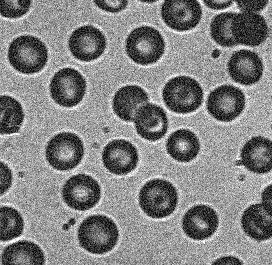
\includegraphics[width=5cm]{bloodCells.png}}

 \caption{Sobel derivative filter.}
 \label{fig:introduction:matlab:sobel}
\end{figure}

\subsection{Enhancement filters}
This quite simple method is used in photo manipulation softwares in order to artificially increase the focus of an image. The human visual perception  positively responds to this type of filter.
\begin{matlab}
B=imread('osteoblaste.bmp');
B=double(B);
B=B/255;
hlaplacien=[-1 -1 -1; -1 8 -1;-1 -1 -1];
Blaplacien=imfilter(B,hlaplacien);
Benhance1=B+Blaplacien;
Benhance2=0.5*B+Blaplacien;
Benhance3=2*B+Blaplacien;
figure
subplot(221);imshow(B);title('Original');
subplot(222);imshow(Benhance1);title('Enhancement : 1');
subplot(223);imshow(Benhance2);title('Enhancement : 0.5');
subplot(224);imshow(Benhance3);title('Enhancement : 2');
\end{matlab}

\begin{figure}[htbp]
 \centering
 
 \subfloat[$\alpha=1$.]{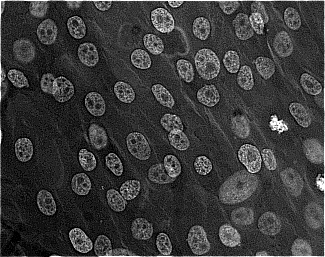
\includegraphics[width=5cm]{osteoblasts_rehauss_1.png}}
 \hspace{1cm}
 \subfloat[$\alpha=0.5$.]{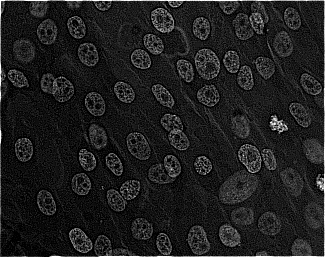
\includegraphics[width=5cm]{osteoblasts_rehauss_0_5.png}}
 
 \subfloat[$\alpha=2$.]{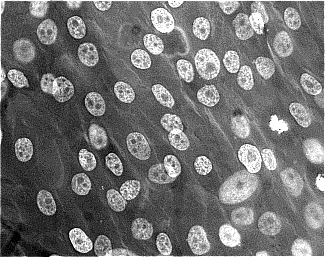
\includegraphics[width=5cm]{osteoblasts_rehauss_2.png}}
 \hspace{1cm}
 \subfloat[Original image.]{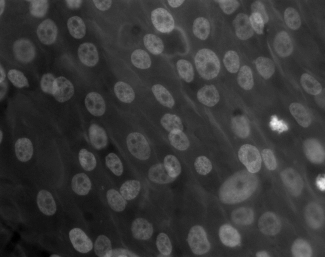
\includegraphics[width=5cm]{osteoblaste.png}}

 \caption{Image enhancement: $I=\alpha\cdot I+HP(I)$, where $HP$ is a high-pass filter (the Laplacian filter in these illustrations).}
 \label{fig:introduction:matlab:enhancement}
\end{figure}

\subsection{Open question}
The histogram equalization is a method that will further developped. The result is presented in Fig.\ref{fig:introduction:matlab:histeq}.

\begin{matlab}
figure
Bhisteq=histeq(B);
subplot(131);imshow(B);title('original image');
subplot(132);imshow(Benhance3);title('enhancement by laplacian');
subplot(133);imshow(Bhisteq);title('histogram equalization enhancement);
\end{matlab}

\begin{figure}[htbp]
\centering
 \subfloat[Original image.]{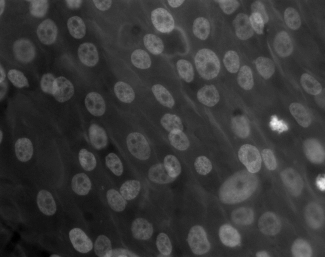
\includegraphics[width=5cm]{osteoblaste.png}}
 \hspace{1cm}
 \subfloat[Histogram equalization.]{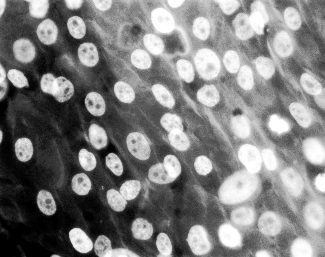
\includegraphics[width=5cm]{osteoblasts_histeq.png}}

 \caption{Image enhancement by histogram equalization. When extreme intensity values are present in a image (white or black values), histogram stretching is useless. The histogram equalization can thus be a solution in order to enhance the image.}
 \label{fig:introduction:matlab:histeq}
\end{figure}

